\chapter{Design}
Angelina Scheler \& Christian Pfeiffer

\section{Einleitung}
Aufgabe des Design Teams war das Design der Stundenplanapp zu überarbeiten und zu verbessern, unter Berücksichtigung der Apple Human Interface Design Guideline. Dabei wurden für die V4 folgende Ziele gesetzt:

\begin{itemize}
\item Verbesserung der Stundenplanansicht
\item Design eines Onboarding Assistenten
\item Verbesserung und Vereinfachung der Einstellungen
\item Design eines Widgets
\end{itemize}


\section{Stundenplan}
Die Ansicht des Stundenplans ist das primäre Feature unserer Stundenplanapp. Deshalb ist es besonders wichtig, dieses stetig zu verbessern und zu erweitern.
Deshalb haben wir, um das Layout übersichtlicher zu gestalten, verschiedene Designkonzepte entworfen.

\subsection{Vorschlag zur Verbesserung der Usability der Stundenplanansicht}
Zu Beginn des Semesters wurde ein Konzept entwickelt, innerhalb dessen die Stundenplanfunktion durch eine Wochenansicht erweitert werden sollte. 

\begin{figure}[H]
	\centering
  \frame{ 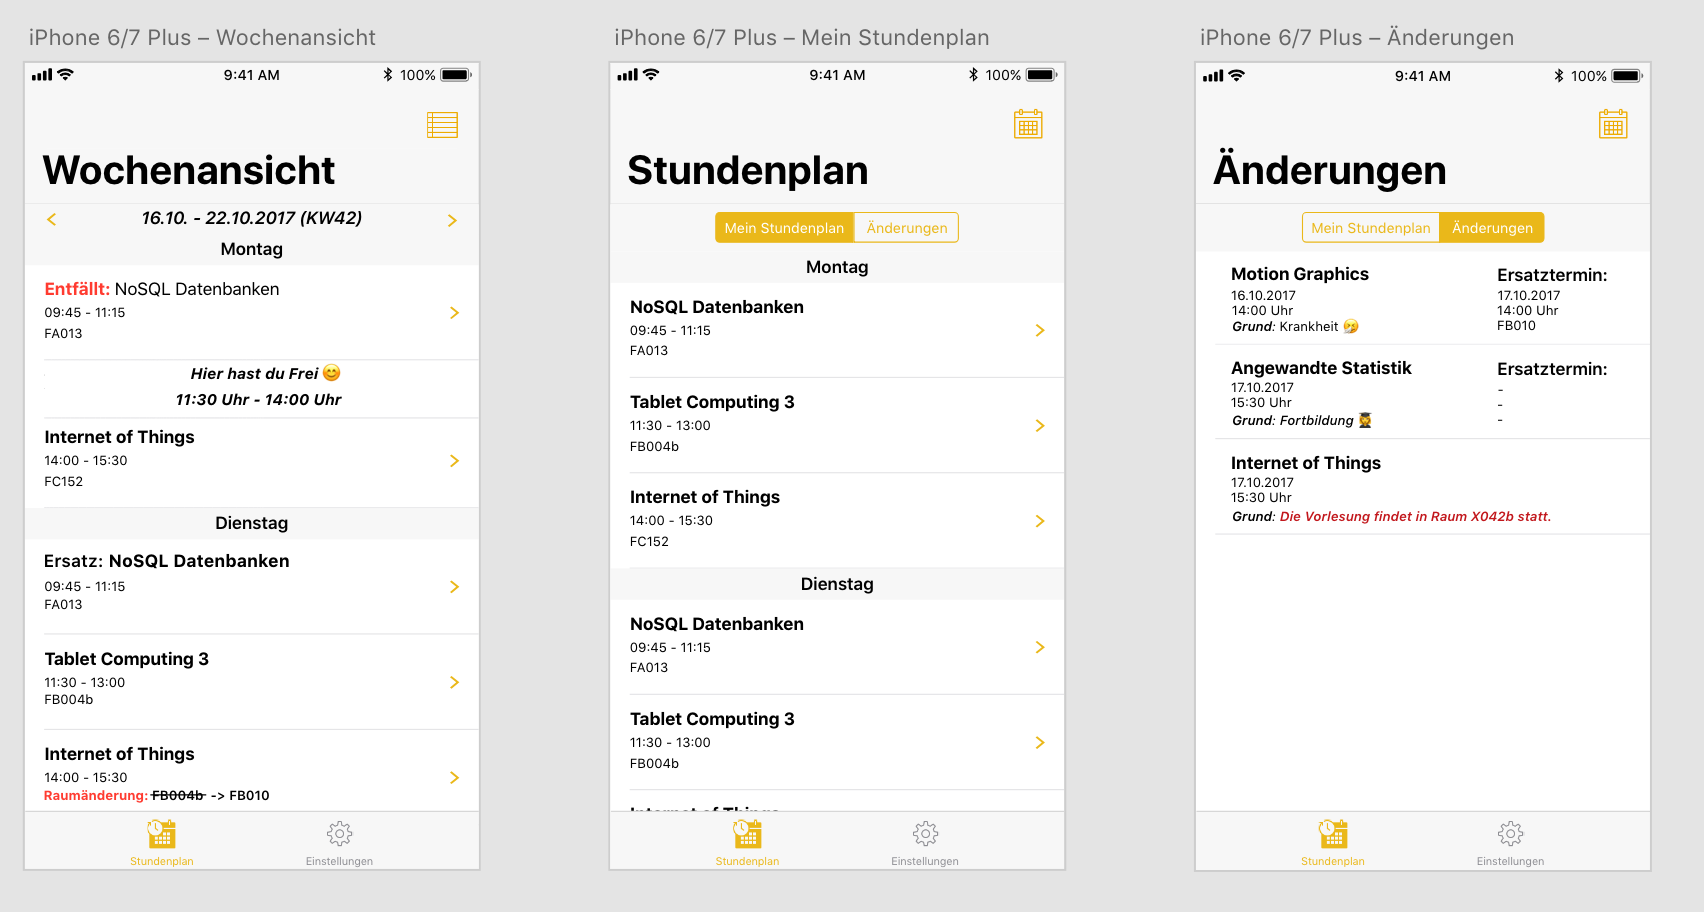
\includegraphics[scale=0.5]{design_stundenplan}}
	\caption{Neues Stundenplanbedienkonzept}
	\label{fig1}
\end{figure}

Mit dem rechten oberen Navigationitem kann zwischen einer Wochenansicht und der klassischen Stundenplanansicht gewechselt werden. In der klassischen Stundenplanansicht kann der Benutzer durch ein ein Segmented Control Element unterhalb der Navigationbar zwischen 'Mein Stundenplan'' und den Stundenplanänderungen wechseln. In der Wochenansicht werden ''Mein Stundenplan'' und die Stundenplanänderungen in einer Ansicht für die aktuelle Woche kombiniert dargestellt. 

\subsection{Entwicklung eines neuen Farbdesigns mit neuem Layout der Zellen}
In der vorherigen Version der Stundenplanapp hatte jede Funktion eine eigene, dem Hochschulfakultäten entsprechende, Farbe. Da das Wechseln der Farbe, bei Auswahl einer neuen Funktion inkonsistent ist, hat das Designteam ein Konzept entwickelt, durch welches der Appnutzer in den Einstellungen seine Fakultät wählen kann und die App damit mit der gewählten Fakultätsfarbe anpassen kann. 
Die folgenden Abbildungen zeigen die Stundenplanansicht in den jeweiligen Fakultätsfarben. Das Layout der Stundenplanzellen wurde darüber hinaus auch verbessert. 

\begin{figure}[H]
	\centering
  \frame{ 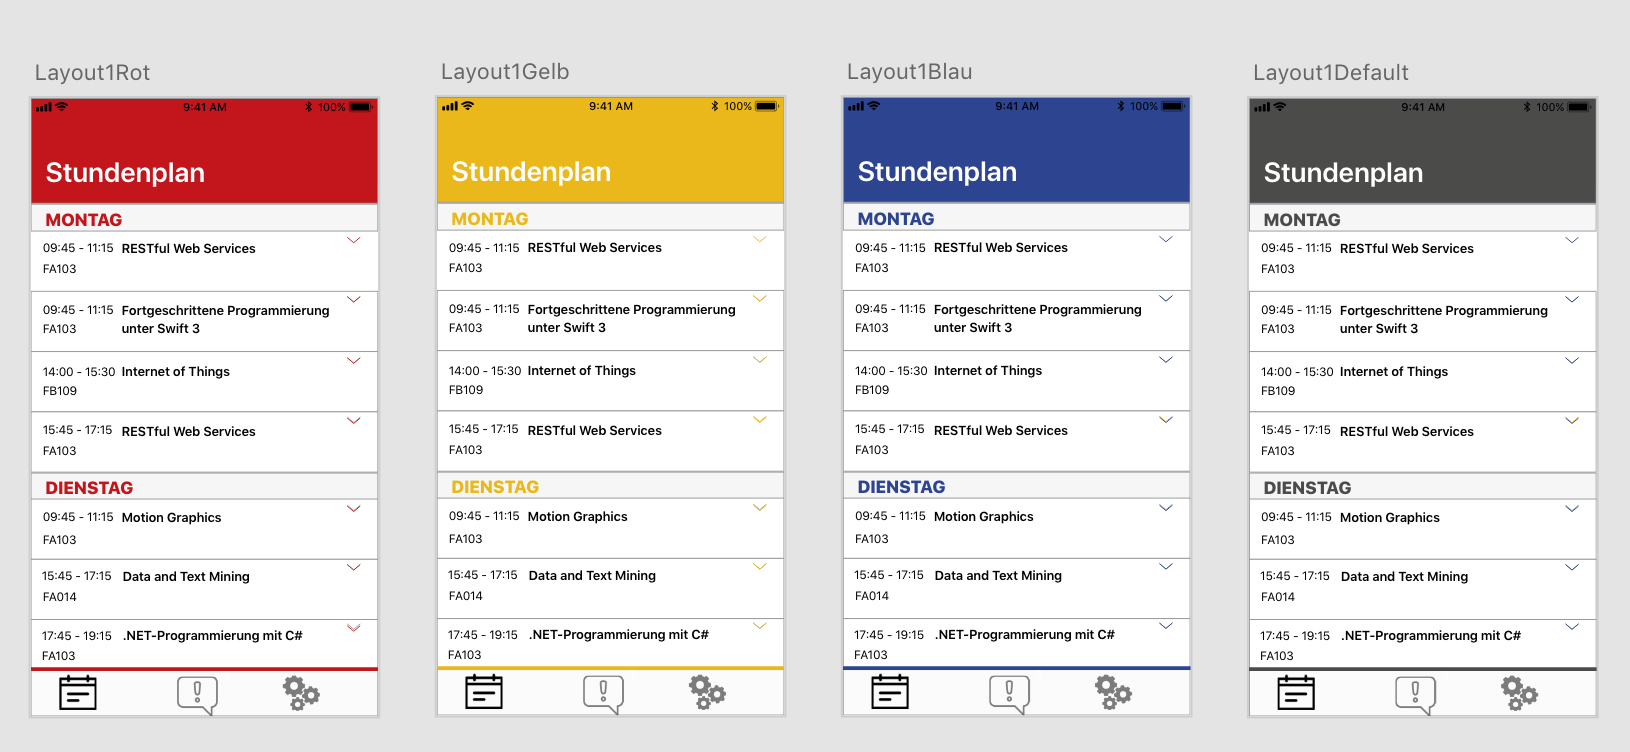
\includegraphics[scale=0.5]{Design1}}
	\caption{Design Konzept 1, Stundenplan Ansicht}
	\label{fig1}
\end{figure}

\begin{figure}[H]
	\centering
  \frame{ 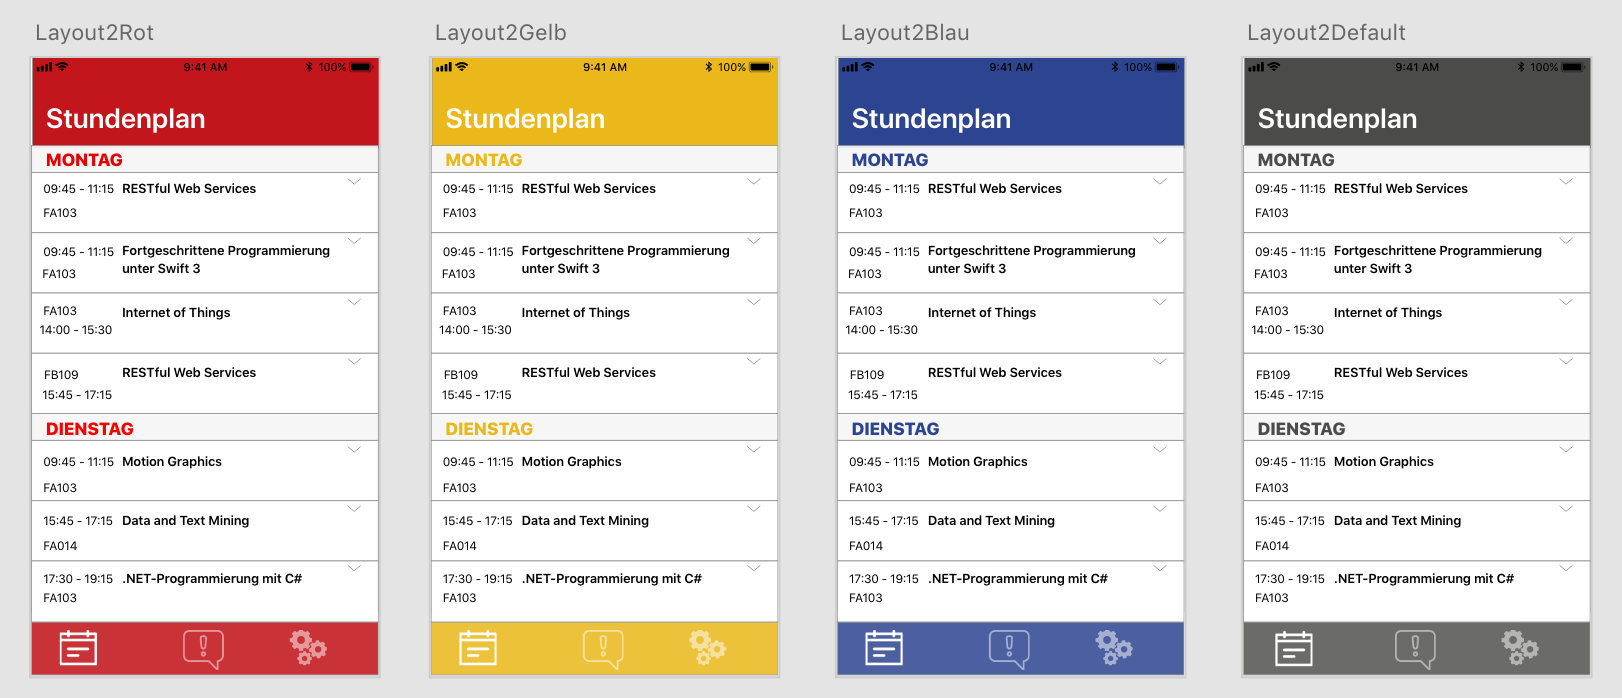
\includegraphics[scale=0.5]{Design2}}
	\caption{Design  Konzept 2, Stundenplan Ansicht}
	\label{fig1}
\end{figure}

\begin{figure}[H]
	\centering
  \frame{ 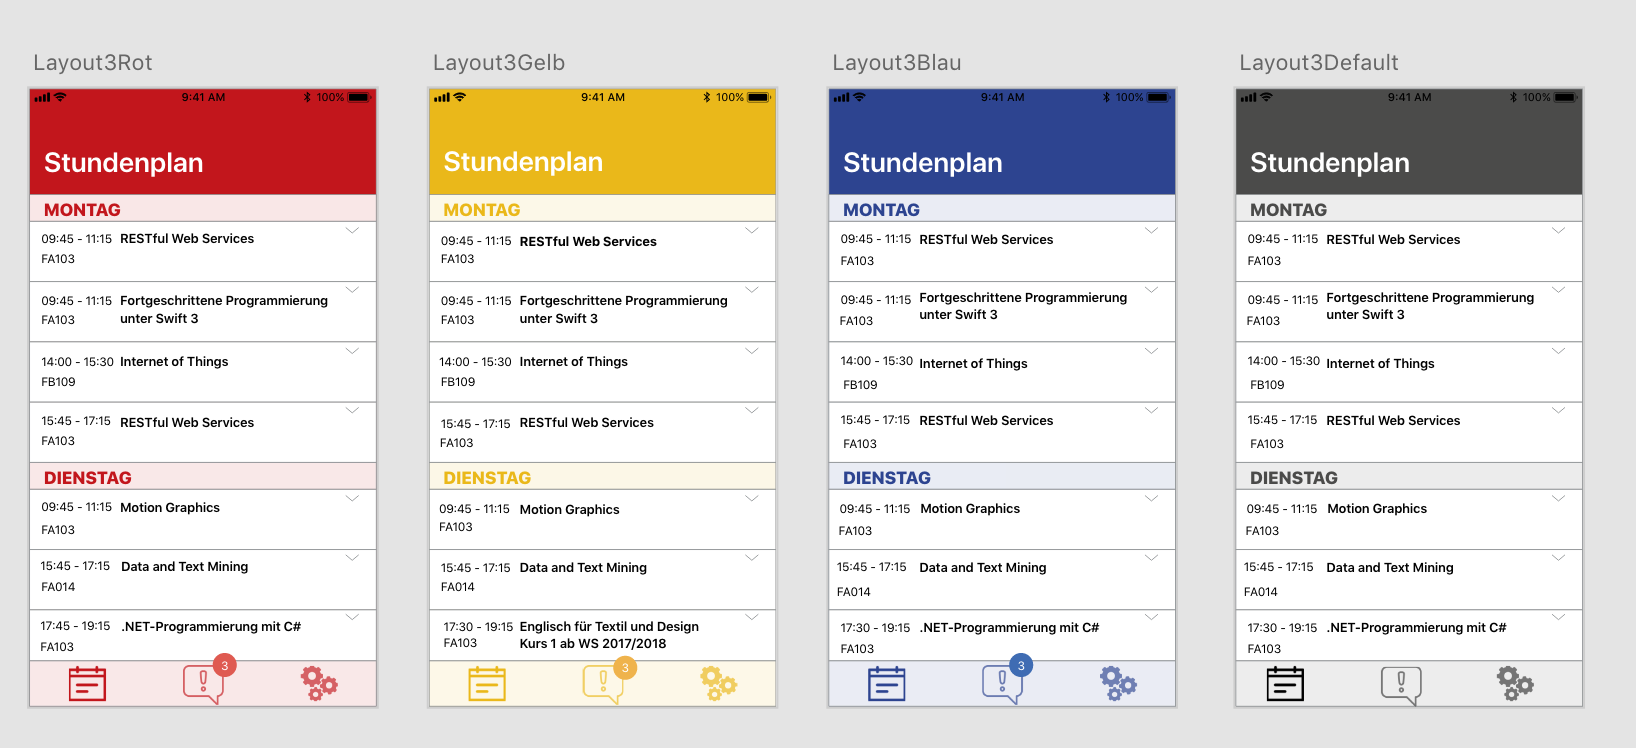
\includegraphics[scale=0.5]{Design3}}
	\caption{Design Konzept 3,  Stundenplan Ansicht}
	\label{fig1}
\end{figure}

\begin{figure}[H]
	\centering
  \frame{ 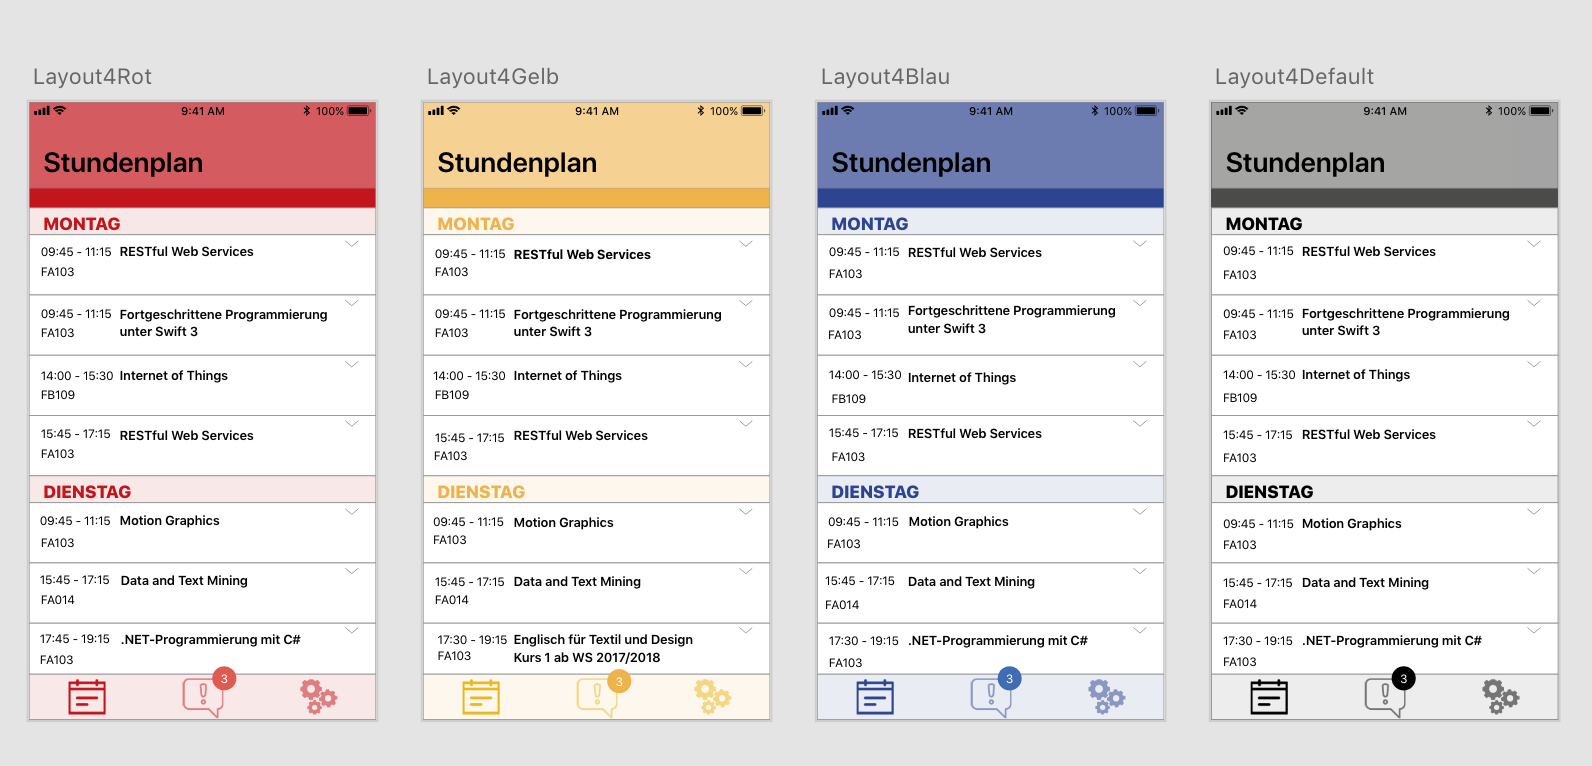
\includegraphics[scale=0.5]{Design4}}
	\caption{Design Konzept 4,  Stundenplan Ansicht}
	\label{fig1}
\end{figure}

\subsection{Finales Design}
Das Finale Design ist ein Kompromiss aus Altem und Neuem Layout, die Fakultätsfarben wurden eingeführt, Informationen übersichtlicher positioniert und farblich angepasst.

\begin{figure}[H]
	\centering
  \frame{ 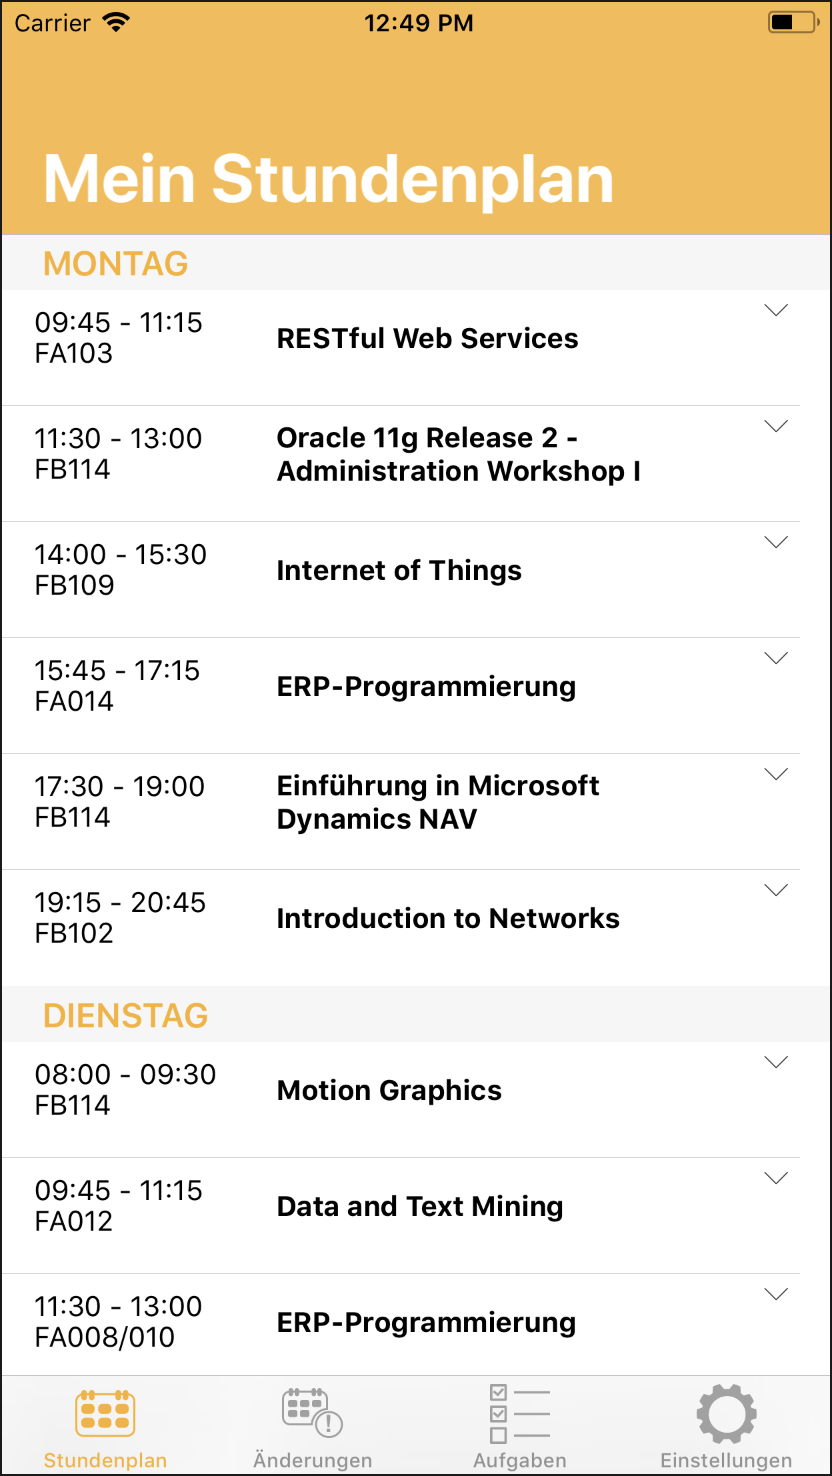
\includegraphics[scale=0.5]{FinalesDesignStundenplan}}
	\caption{Finales Design, Stundenplan Ansicht}
	\label{fig1}
\end{figure}

\begin{figure}[H]
	\centering
  \frame{ 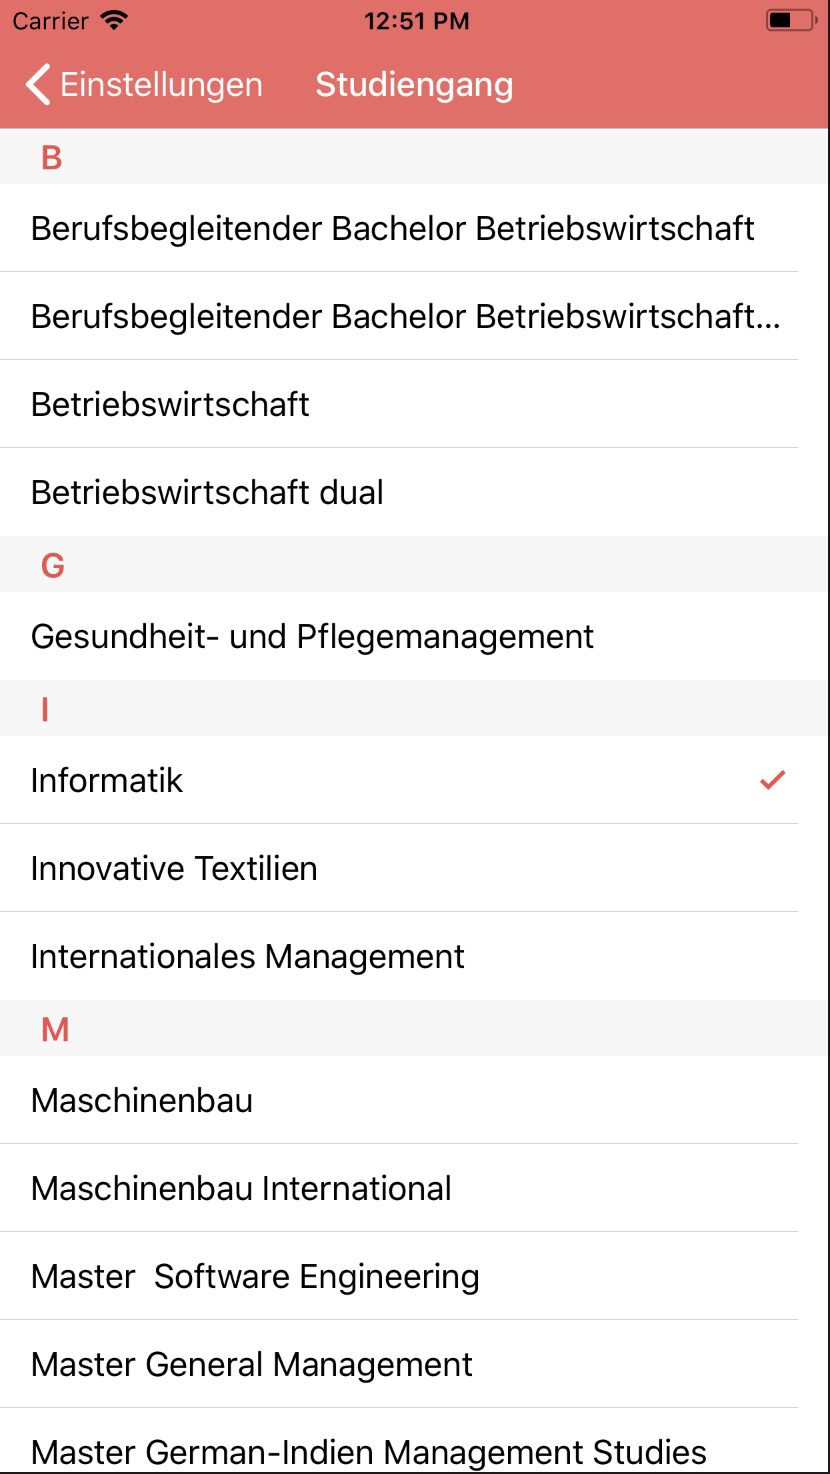
\includegraphics[scale=0.5]{DesignAuswahlStudiengang}}
	\caption{Finales Design, bsp. Auswahl Studiengänge}
	\label{fig1}
\end{figure}




\section{Onboarding}

Um neuen Appnutzern eine geführte Einführung in die Funktionalität und Einstellungsmöglichkeiten zu bieten, ist die Implementation einer Onboardingfunktion sinnvoll. Deshalb wurden Mockups einer solchen Funktion entwickelt, die einen solchen Onboardingprozess darstellen.

\begin{figure}[H]
	\centering
  \frame{ 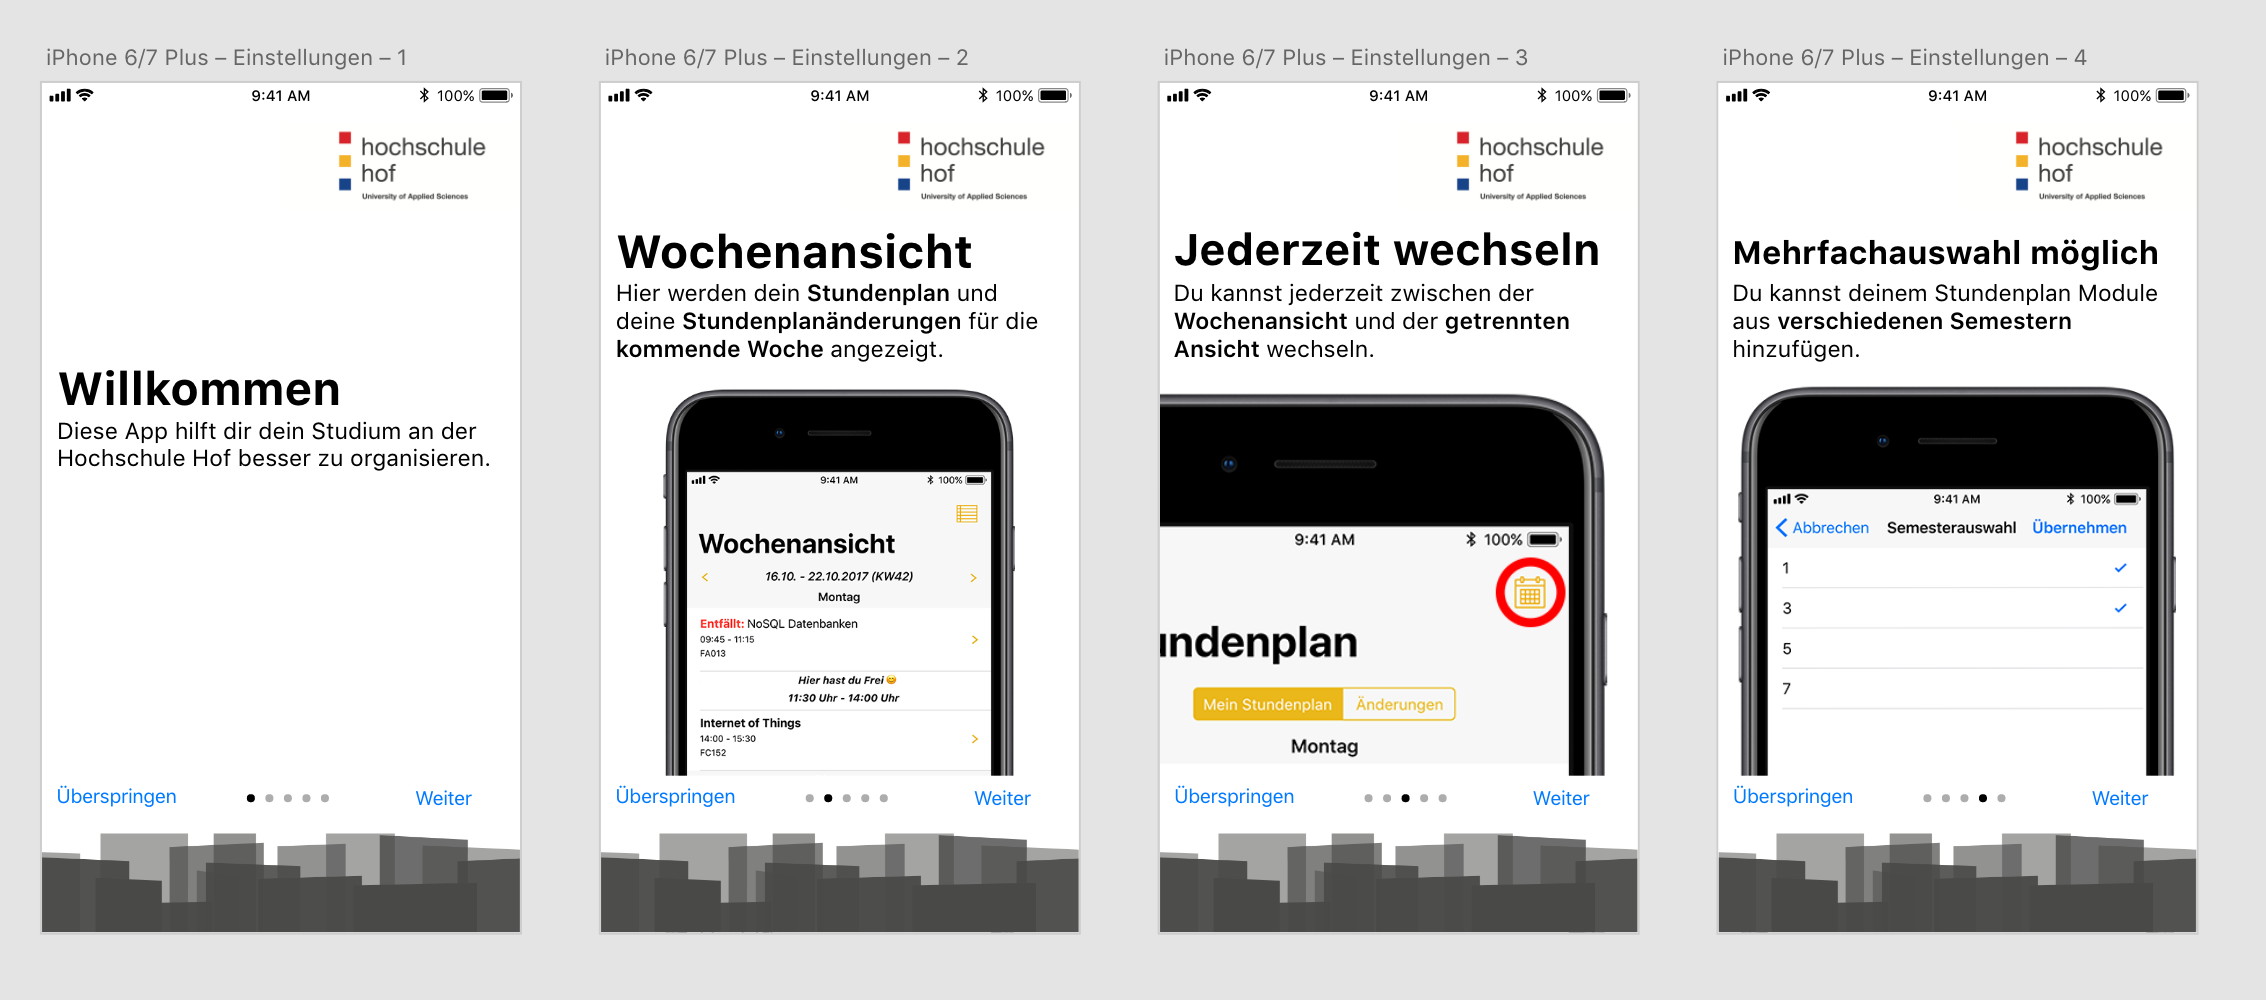
\includegraphics[scale=0.4]{design_onboarding1}}
	\caption{Neues Stundenplanbedienkonzept}
	\label{fig1}
\end{figure}

\begin{figure}[H]
	\centering
  \frame{ 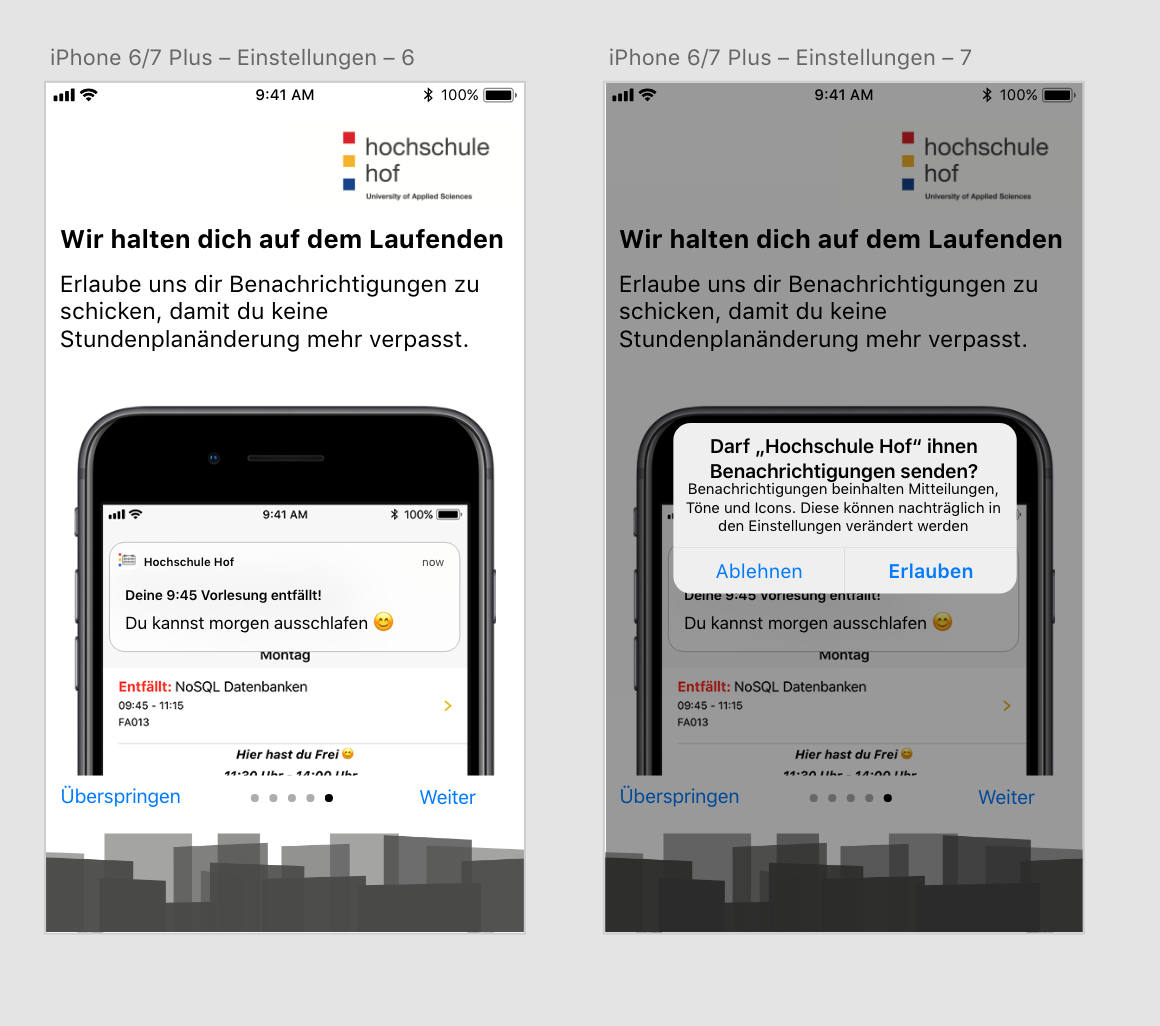
\includegraphics[scale=0.5]{design_onboarding2}}
	\caption{Neues Stundenplanbedienkonzept}
	\label{fig1}
\end{figure}


\section{Einstellungen}
Das Einrichten der App unter Einstellungen sollte durch eine übersichtlichere Gestaltung vereinfacht werden. 

\subsection{Vereinfachung der Stundenplanauswahl}
In der vorherigen Versionen der Stundenplanapp, war die Auswahl eines persönlichen Stundenplans 

\begin{figure}[H]
	\centering
  \frame{ 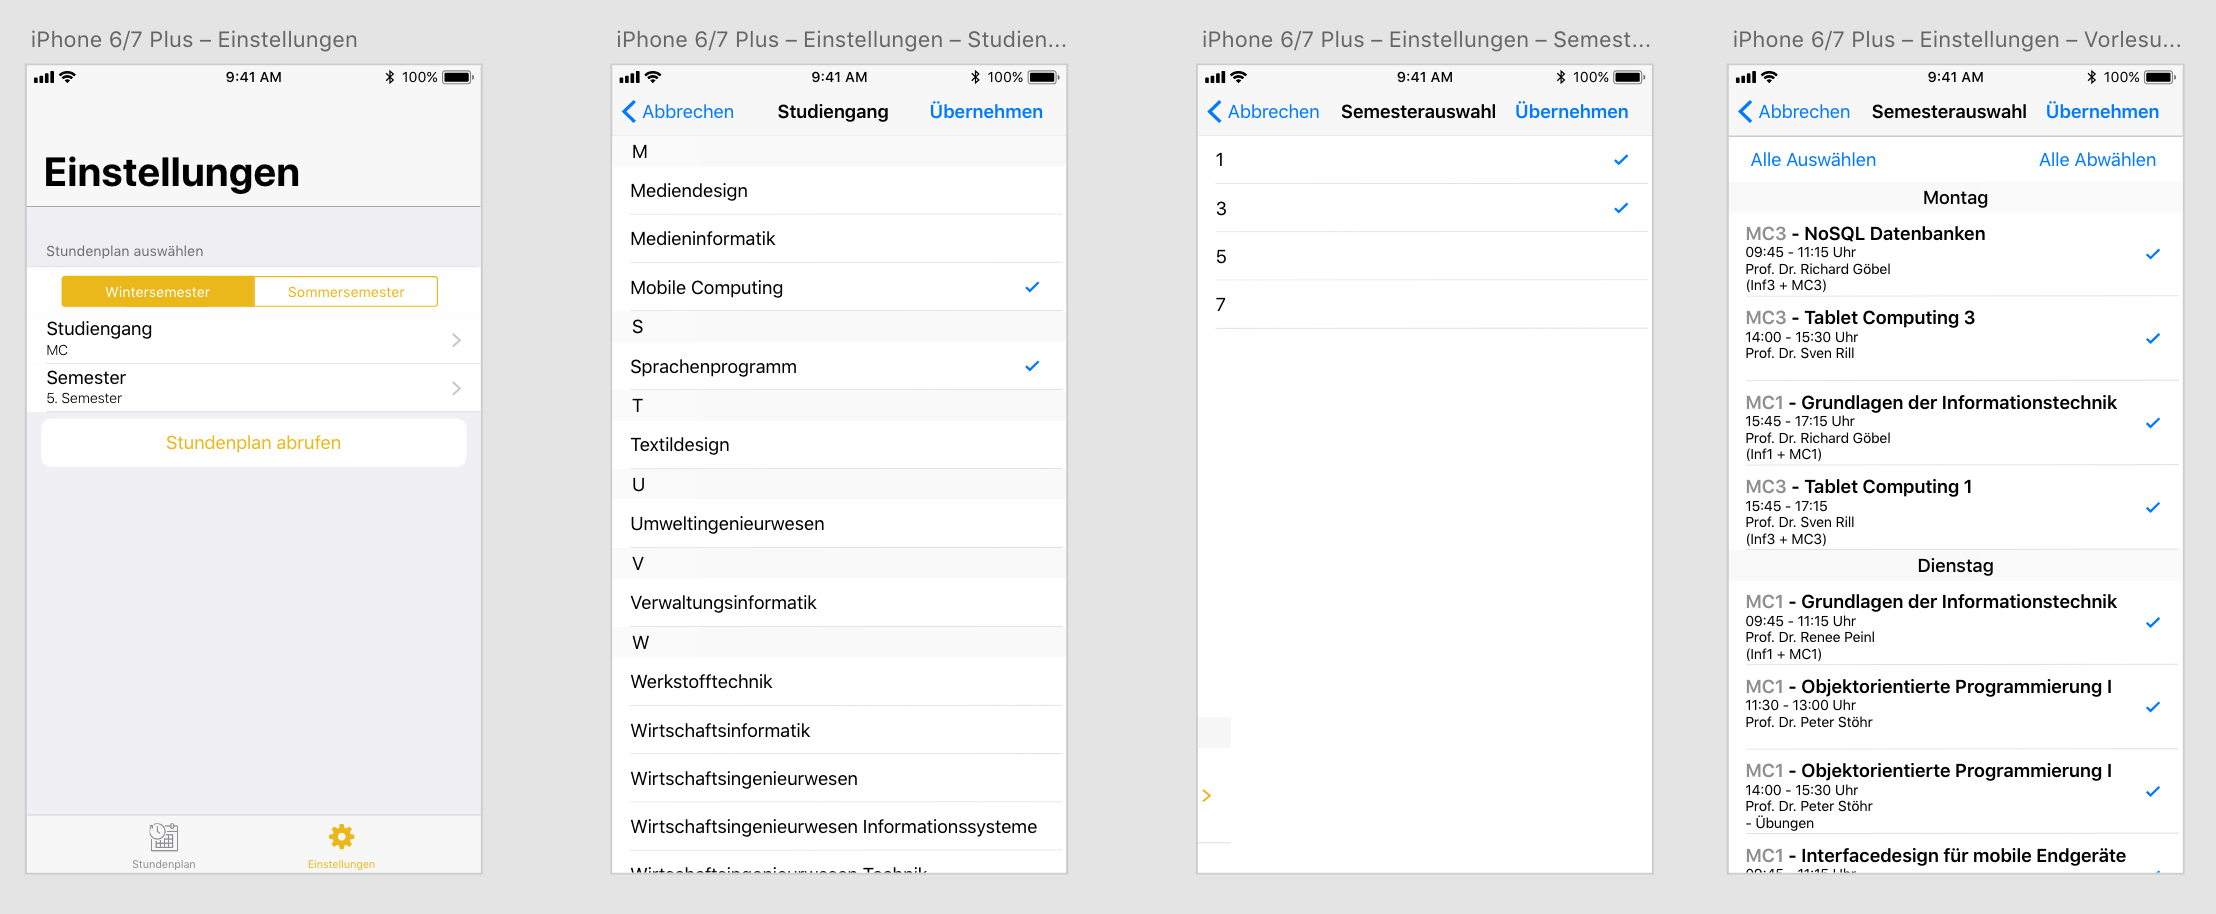
\includegraphics[scale=0.5]{design_settings}}
	\caption{Optimierung der Schritte zur Stundenplanauswahl auf die nötigsten Schritte}
	\label{fig1}
\end{figure}

\subsection{Design Vorschlag}

\begin{figure}[H]
	\centering
  \frame{ 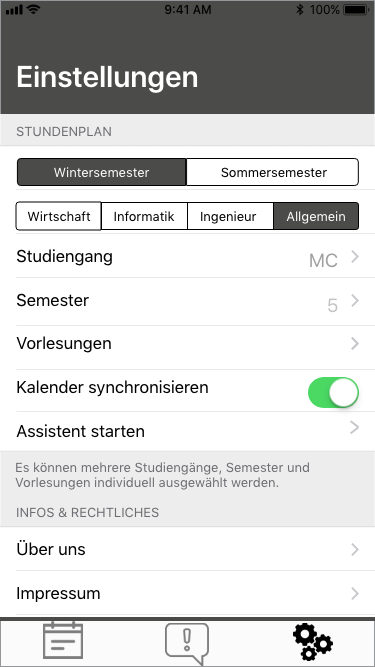
\includegraphics[scale=0.5]{Layout1Settings}}
	\caption{Design Konzept, Stundenplan Einstellungen}
	\label{fig1}
\end{figure}

\subsection{Design Umsetzung}
Es wurde ein Menüpunkt für die Fakultätsauswahl und starten des Einführungsassistenten eingefügt. Desweiteren wurden in den jeweiligen Einstellungsscreens wie, Studiengang, Semester und Vorlesungen anpassungen vorgenommen, wie die Alphabetisierung siehe Abbildung 2.8.. Außerdem wurden alle Inhalte je nach Fakultätsauswahl farblich angepasst.

\begin{figure}[H]
	\centering
  \frame{ 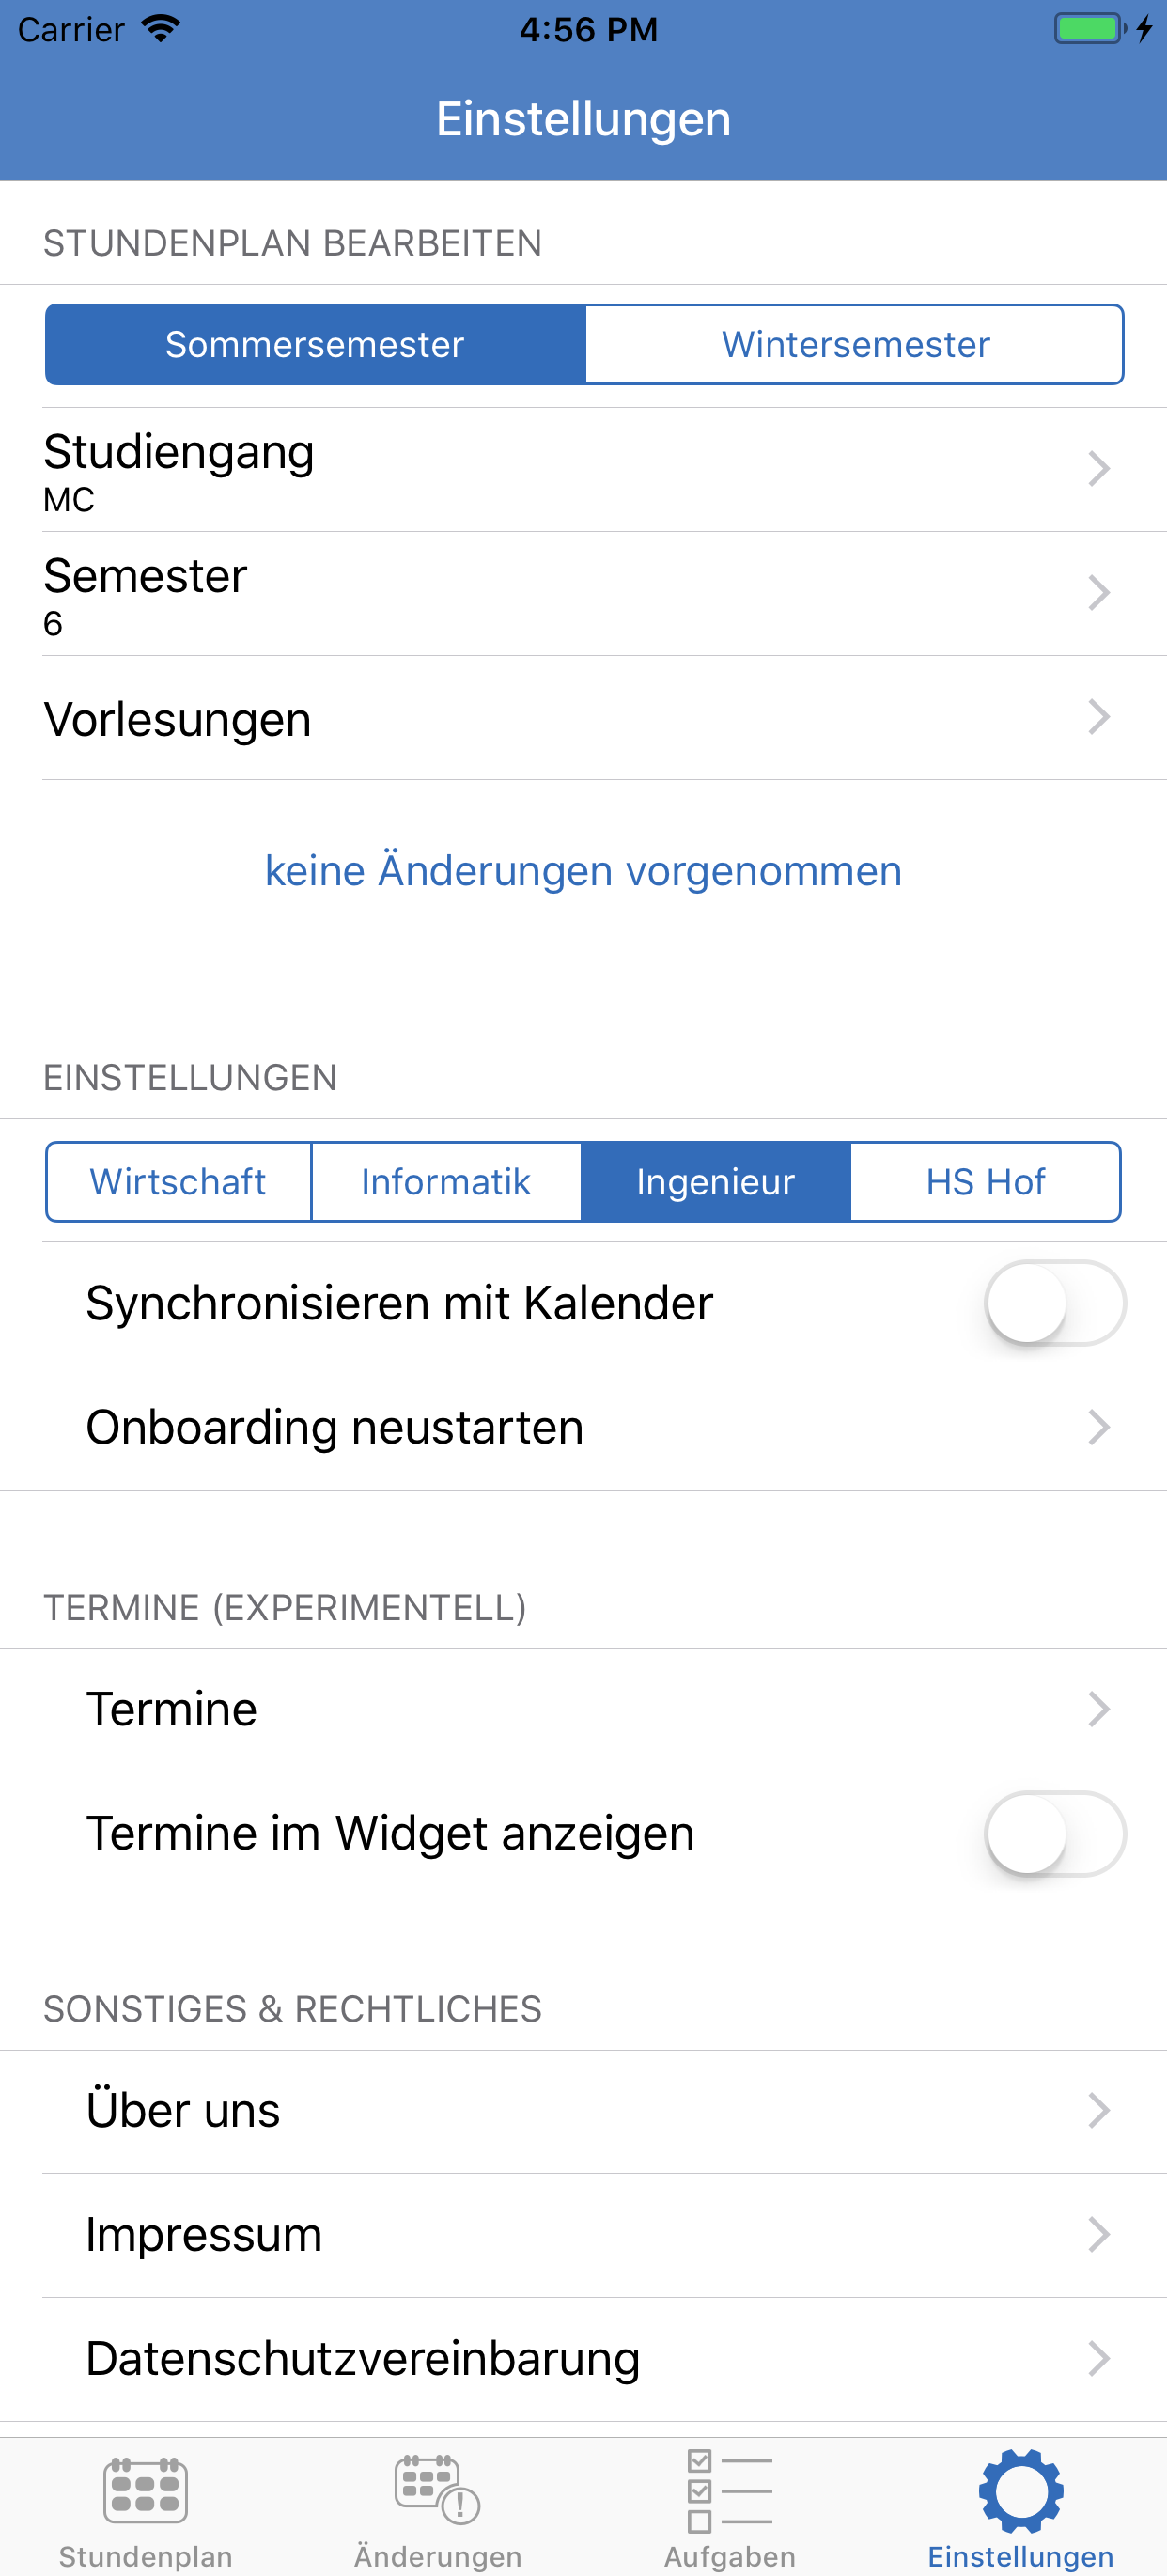
\includegraphics[scale=0.5]{FinalesDesignSettings}}
	\caption{Finales Design, Stundenplan Einstellungen}
	\label{fig1}
\end{figure}

\begin{figure}[H]
	\centering
  \frame{ 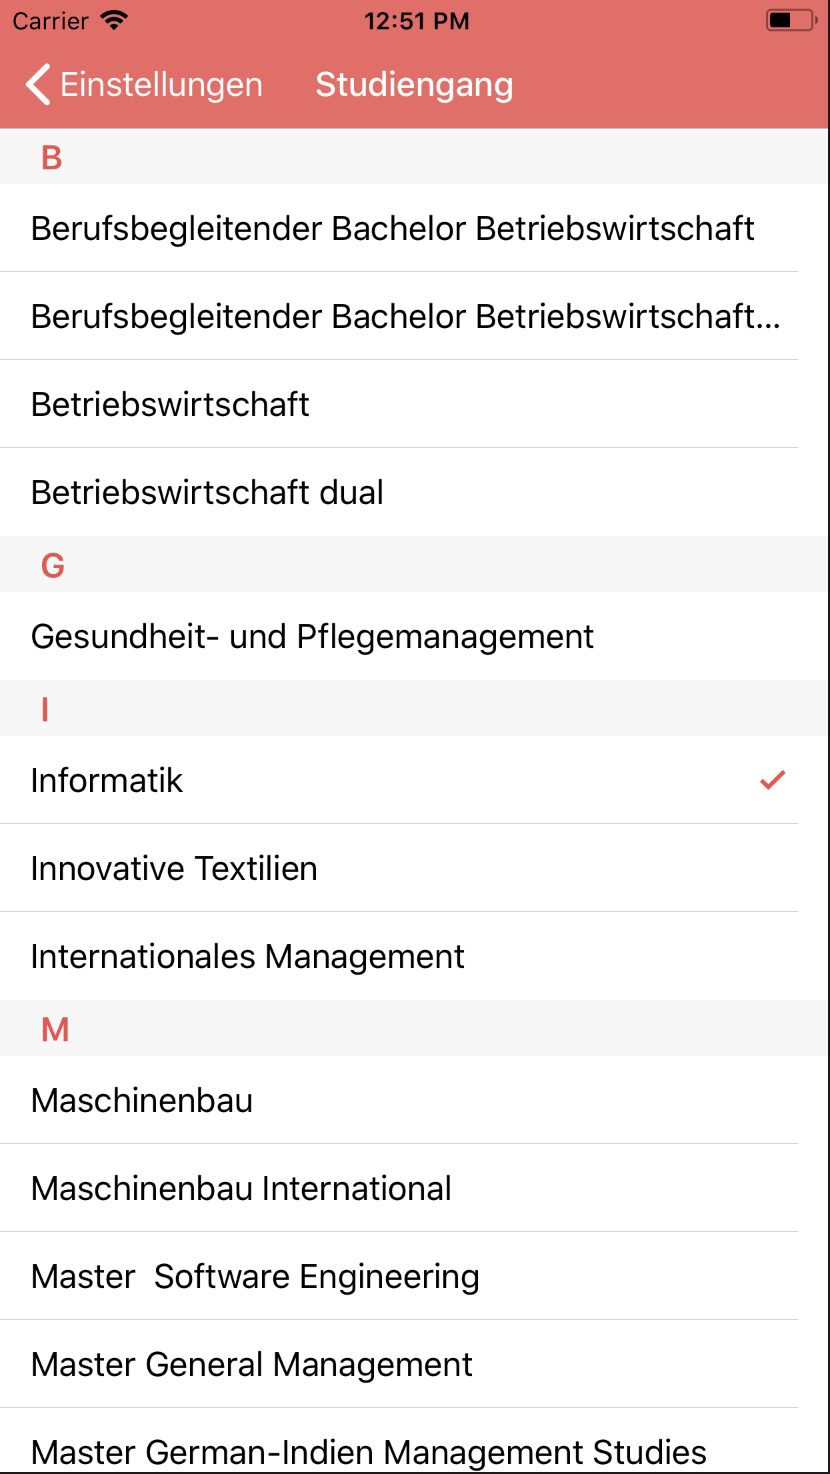
\includegraphics[scale=0.5]{DesignAuswahlStudiengang}}
	\caption{Finales Design, bsp. Auswahl Studiengänge}
	\label{fig1}
\end{figure}

\section{Widget}

\subsection{Design Vorschlag}

\begin{figure}[H]
	\centering
  \frame{ 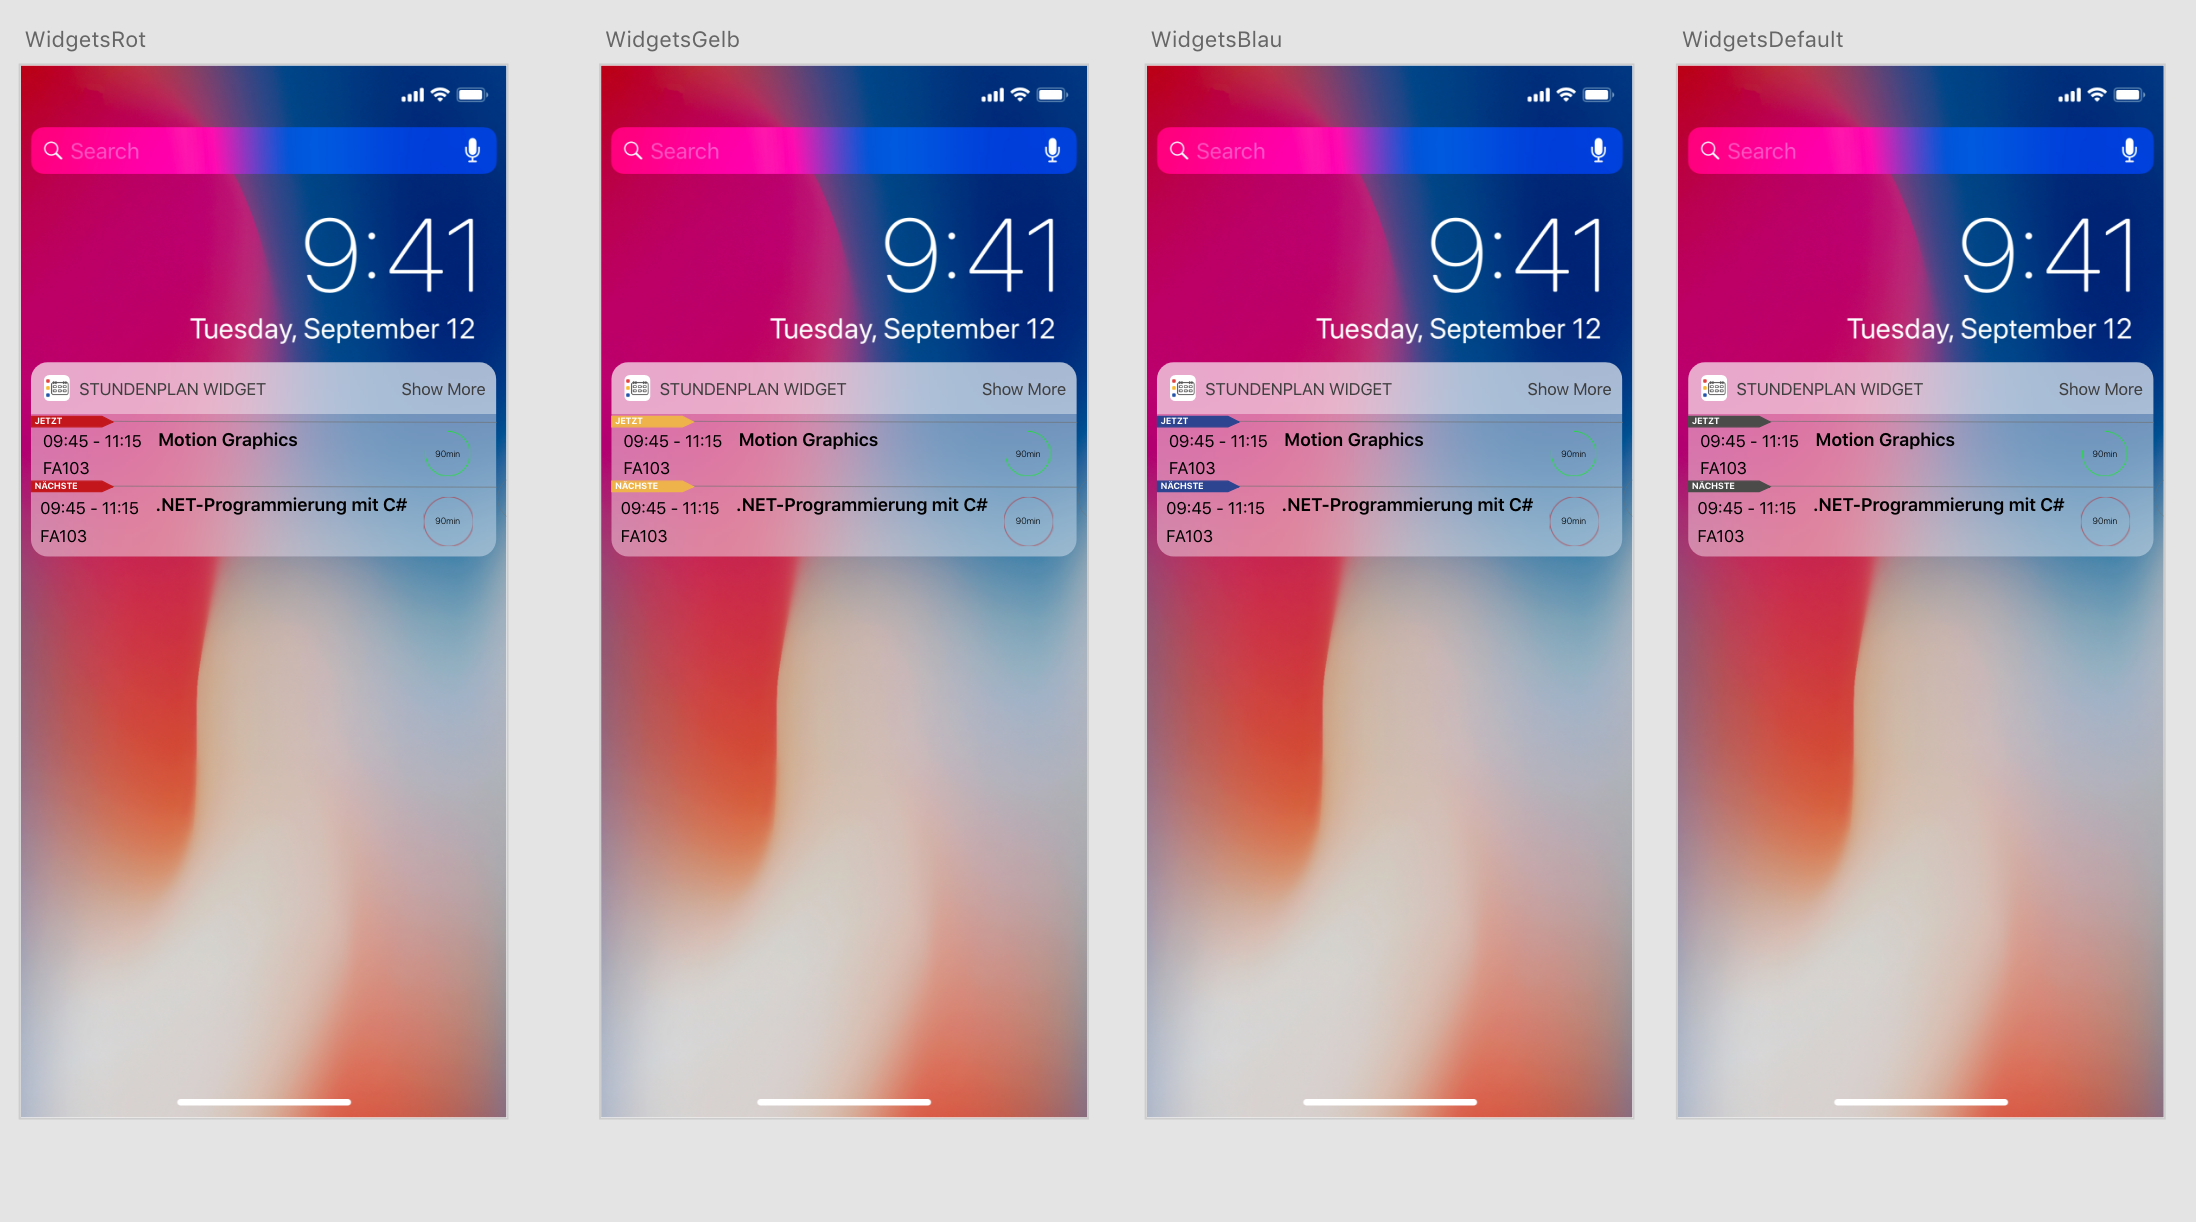
\includegraphics[scale=0.5]{WidgetDesign}}
	\caption{Design Vorschlag, Widget}
	\label{fig1}
\end{figure}




\section{demo}
Eine weitere Aufgabe, die unsere Gruppe übernommen hat, war das Onboarding für die Stundenplan App. Im Onboarding kann der Nutzer gleich zum Start der App seine Einstellungen zu Fakultät, Studiengang, Semester, Vorlesung und Kalendersynchronisation vornehmen. Das Onboarding wird gestartet, wenn noch keine Angaben zu den genannten Einstellungen gemacht wurden.

\begin{itemize}
\item Neues Design
\item besseres Design
\item iOS Design
\end{itemize}

\begin{enumerate}
\item Fakultät (die die Farbe der App bestimmt)
\end{enumerate}

\begin{figure}[H]
	\centering
  \frame{ 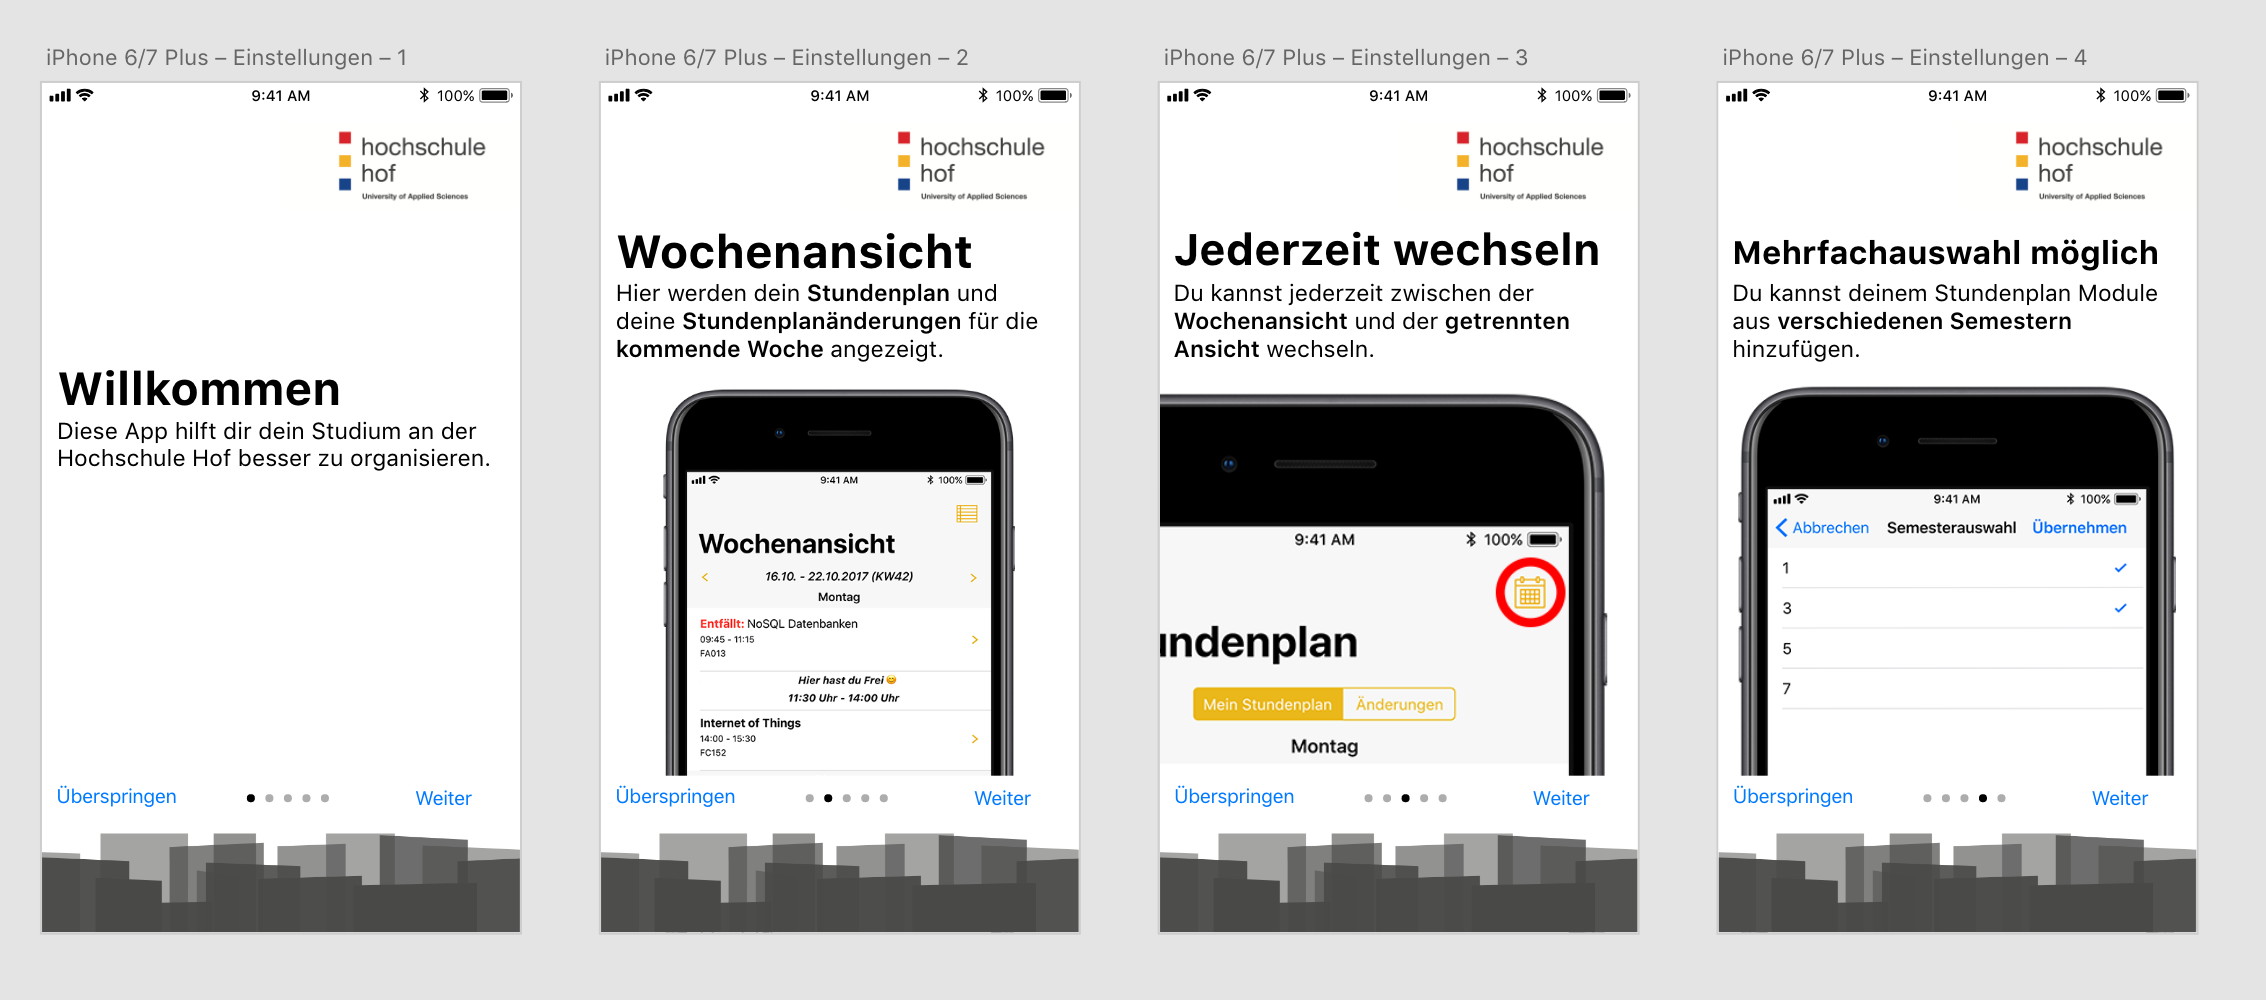
\includegraphics[width=0.3\textwidth]{design_onboarding1} }
	\caption{Mein schönstes Mockup}
	\label{fig2}
\end{figure}

